\documentclass[a4paper]{article}

%% Language and font encodings
\usepackage[english]{babel}
\usepackage[utf8x]{inputenc}
\usepackage[T1]{fontenc}

%% Sets page size and margins
\usepackage[a4paper,top=3cm,bottom=2cm,left=3cm,right=3cm,marginparwidth=1.75cm]{geometry}

%% Useful packages
\usepackage{amsmath}
\usepackage{graphicx}
\usepackage[colorinlistoftodos]{todonotes}
\usepackage[colorlinks=true, allcolors=blue]{hyperref}

\title{Generating natural language with deep generative models (AKA. Project Neo)}
\author{Hamidreza Saghir}

\begin{document}
\maketitle


\section{Motivation}

Machine learning and data science in general are concerned with discovering patterns and insights in large collections of data. The advent of deep learning models in particular, have had a major impact on many task in computer vision and natural language processing as well as other domains. In essence, machine learning models condense the information contained in raw data into a machine representation, from which insights are extracted and communicated to provide business and scientific value.

Language is the primary facet of communication for humans. Communicating insights from a machine representation back into human language is critical for making the findings accessible and providing value. Natural language generation (NLG) is the task of automatically generating human language from a machine representation of data e.g. a knowledge graph. Systems that can perform NLG may be able to communicate hard to understand machine representations of relationships in the data to human language and therefore act as a layer on top of machine learning models for communication of findings to humans.

\section{Objective}
The long-term vision for the "Neo" project is to bridge the gap between machine representation and human understanding. This vision can include explainable and interpretable machine learning given availability of proper settings and datasets, however, the short term objective is to build a human language generation engine that can be used for communicating relationships. 

Such language generation engines are particularly very important in business contexts where the end-users of machine learning products are usually non-technical and require human language communication to be able to gain value from machine learning products. 

\section{The case of the Apollo project}
An example of the immediate value that Neo can provide is project Apollo, a news understanding engine that processes vast amount of textual articles to find relationships between entities and encode them into a knowledge graph representation. While Apollo extracts entities and events from many news articles and represents them in a graph, Neo translates back the found relationships into human language. Therefore Neo will act as a a layer on top of Apollo project that connects it to humans and users.

A possible set of end-users for Apollo are financial market analysts that rely on news articles and other information about the real world to form investment strategies. In a recent consultation with a group of financial analysts, the Apollo team found that analysts would benefit more from a set of statements about the real-world in human language. Neo can provide this missing link and help analysts understand the information contained in the Apollo knowledge graph in the form of human language statements.

\subsection{Dataset}
Apollo currently uses the Thomson-Reuters news articles dataset and builds a knowledge graph to represent the information contained in the articles about entities and their relationships. Such a dataset is the perfect setup for Neo to add value due to the availability of textual data for training language generation models and the knowledge graph representation of the same text for relationships that require translation back into human language.

An example of the relationship between textual data and the knowledge graph of the Apollo project are relationships like this:
\begin{itemize}
  \item sentence [GM invests 500MM in Lyft] $\to$ knowledge graph representation [nodes(GM, Lyft), relationship(investing)]
  \item $\to$ possible generated statement [GM invests in Lyft]
\end{itemize}
 
The idea is to train a language model conditioned on the knowledge graph to generate human readable sentences and statements about the relationships between entities.

\section{Methodology}
\subsection{Variational Autoencoder}
A variational autoencoder (VAE) (Figure \ref{fig:vae}:Left) is a latent variable model that uses deep neural networks to represent conditional distributions. VAEs use the autoencoding variational Bayes framework [1] for learning the inference and generative network at the same time using stochastic gradient descent. VAEs are based on the re-parameterization trick that disentangles the stochastic and deterministic part of the latent random variable in the model. This enables passing of gradients through the latent variable to be able to learn both the inference and generative networks end-to-end simultaneously. 

A conditional VAE [2] (Figure \ref{fig:vae}: Right) is similar to a vanilla VAE model with the difference that the graphical model includes an additional observed variable which provides a condition for the generative network to use for producing observations. A conditional VAE is useful for adding additional constraints to the generative process and providing a control nob for data generation. 

\begin{figure}
\centering
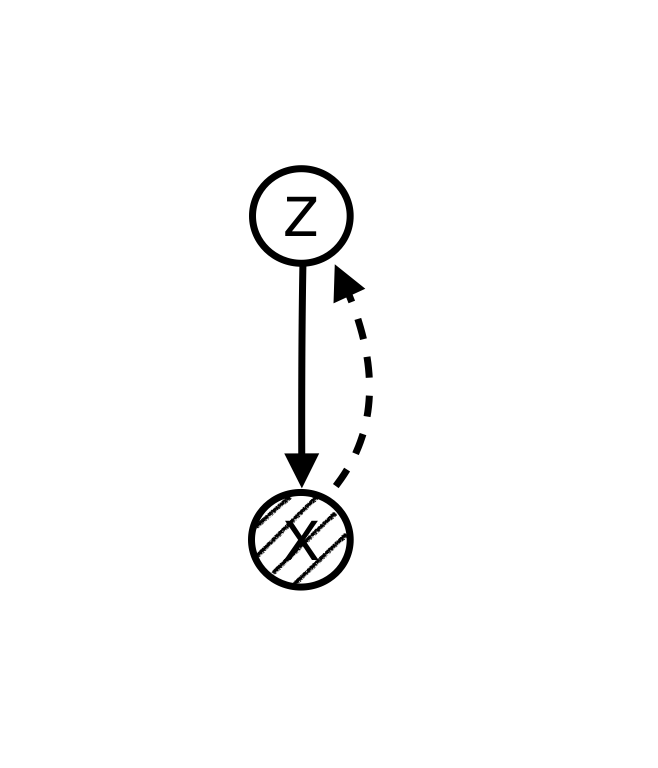
\includegraphics[width=0.3\textwidth]{vanilla_vae.png} | 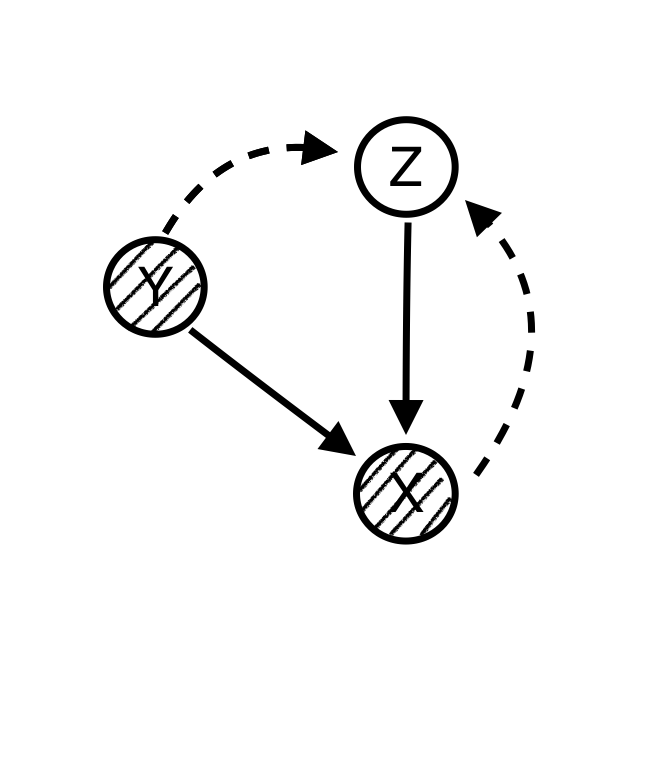
\includegraphics[width=0.3\textwidth]{cvae.png} 
\caption{\label{fig:vae}Left: A vanilla VAE graphical model. Right: A conditional VAE graphical model}
\end{figure}

A VAE can be adapted to textual context by using LSTM networks [3] inside both the encoder and decoder of the VAE (Figure \ref{fig:rvae}). This model would be very similar to seq-to-seq [4] type of models with the addition of a Gaussian prior on the latent code that regularizes the autoencoder [5]. Additionally, another advantage of having a distribution on the latent code is the possibility of generating text. In this context, if a degenerate distribution is learned for the latent code, the sequence VAE will revert to a seq-to-seq model. The sentence VAE setup can be improved to learn a more disentangled representation for a more controllable text generation process by adding adversarial costs to the generative network part of the VAE [7] (Figure \ref{fig:cvae_gan}). 


\begin{figure}
\centering
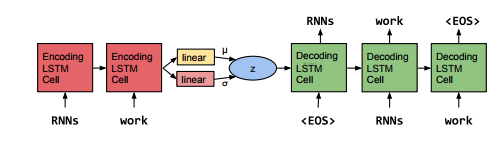
\includegraphics[width=0.3\textwidth]{rvae.png}
\caption{\label{fig:rvae}A sentence VAE setup consisting of LSTM networks in both the inference and generative models.}
\end{figure}


I propose a conditional variational autoencoder with an adversarial objective where  both the encoder and decoder networks employ an LSTM architecture. The decoder part of this network is a generative adversarial network (GAN) that generates a sentence from a condition and noise inputs [17]. To encourage the GAN to effectively use the noise input and avoid the mode collapse problem, the encoder network maps a sentence input into a latent code noise which will be used by the decoder resulting in a more effective use of the noise input by the GAN [16]. This model will be trained on the the Thomson-Reuters dataset and its associated knowledge graph from the Apollo project. This model can be used for conditional generation of text given knowledge graph relationships. In this context, the text generation process is controlled based on the observed relationships in the knowledge graph. 

\begin{figure}
\centering
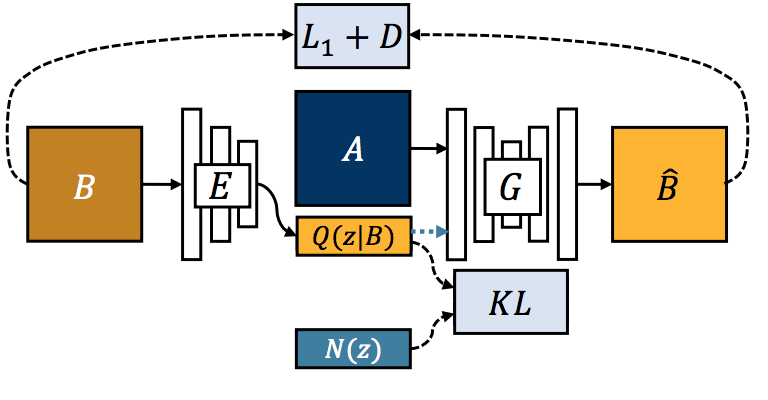
\includegraphics[width=0.3\textwidth]{cvae_gan.png}
\caption{\label{fig:cvae_gan}A conditional VAE model with with adversarial cost}
\end{figure}


\subsection{Discrete variable gradient estimation}
If latent random variables satisfy some conditions and are continuous, they can be re-parameterized to provide a deterministic function where gradients can pass through and enable end-to-end learning of the both the inference and generative networks. However, if the random variables are discrete random variables, which is the case for textual data, then re-parameterization and gradients passing will be much more challenging. This has been particularly challenging in the context of adversarial loss functions. Some recent advances in gradient estimators for discrete variables may provide solutions. Possible gradient estimators for discrete latent variable models include concrete variables [12], vector quantization (VQ) [13],REBAR gradient [14], and RELAX gradient [15]. 


\section{References}

\noindent [1] Kingma, Diederik P., and Max Welling. "Auto-encoding variational Bayes." arXiv preprint arXiv:1312.6114 (2013).

\noindent [2] Kingma, Diederik P., et al. "Semi-supervised learning with deep generative models." Advances in Neural Information Processing Systems. 2014.

\noindent [3] Hochreiter, Sepp, and Jürgen Schmidhuber. "Long short-term memory." Neural computation 9.8 (1997): 1735-1780.

\noindent [4] Sutskever, Ilya, Oriol Vinyals, and Quoc V. Le. "Sequence to sequence learning with neural networks." Advances in neural information processing systems. 2014.

\noindent [5] Bowman, Samuel R., et al. "Generating sentences from a continuous space." arXiv preprint arXiv:1511.06349 (2015).

\noindent [6] Hu, Zhiting, et al. "Controllable Text Generation." arXiv preprint arXiv:1703.00955 (2017).

\noindent [7] Zhou, Chunting, and Graham Neubig. "Multi-space Variational Encoder-Decoders for Semi-supervised Labeled Sequence Transduction." arXiv preprint arXiv:1704.01691 (2017).

\noindent [8] Hsu, Wei-Ning, Yu Zhang, and James Glass. "Unsupervised Learning of Disentangled and Interpretable Representations from Sequential Data." Advances in neural information processing systems. 2017.

\noindent [9] Gupta, Ankush, et al. "A Deep Generative Framework for Paraphrase Generation." arXiv preprint arXiv:1709.05074 (2017).

\noindent [10] Guo, Jiaxian, et al. "Long Text Generation via Adversarial Training with Leaked Information." arXiv preprint arXiv:1709.08624 (2017).

\noindent [11] Ni, Jianmo, et al. "Estimating Reactions and Recommending Products with Generative Models of Reviews." Proceedings of the Eighth International Joint Conference on Natural Language Processing (Volume 1: Long Papers). Vol. 1. 2017.

\noindent [12] Jang, Eric, Shixiang Gu, and Ben Poole. "Categorical reparameterization with gumbel-softmax." arXiv preprint arXiv:1611.01144 (2016).

\noindent [13] van den Oord, Aaron, and Oriol Vinyals. "Neural Discrete Representation Learning." Advances in Neural Information Processing Systems. 2017.

\noindent [14] Tucker, George, et al. "REBAR: Low-variance, unbiased gradient estimates for discrete latent variable models." Advances in Neural Information Processing Systems. 2017.

\noindent [15] Grathwohl, Will, et al. "Backpropagation through the Void: Optimizing control variates for black-box gradient estimation." arXiv preprint arXiv:1711.00123 (2017).

\noindent [16] A. B. L. Larsen, et al. "Autoencoding beyond pixels using a learned similarity metric". In ICML, 2016

\noindent [17] J.Y. Zhu, et al. "Toward Multimodal Image-to-Image Translation". In NIPS, 2017

\noindent [18] Reed, Scott, et al. "Generative adversarial text to image synthesis." arXiv preprint arXiv:1605.05396 (2016).

\end{document}